\part{Confucianisme, Taoïsme et Bouddhisme Chinois}
\chapter{Introduction}

\mn{Jia Bingwei, Doctorante et chargée de cours à l’Université Paris Cité, Collège de France}

\paragraph{spiritualité Chinoise}
Compétences à acquérir à l’issue de l’enseignement :
\item 	Compréhension générale du paysage religieux en Chine dans l’histoire et d’aujourd’hui
\item 	Compréhension des notions de base des traditions religieuses chinoises

\paragraph{objectif } acquérir une vision générale du religieux chinois dans l'histoire et aujourd'hui


\paragraph{une notion centrale : le xiushen chinois}

\begin{Def}[xiushen]
    Apparu au Vè avant JC, cette notion est :
    \begin{itemize}
        \item \textit{taillé}, \textit{corrigé}
        \item shen : le corps
    \end{itemize}
    idée de se perfectionner sans arrêt
\end{Def}

\paragraph{se dépasser à travers certaines pratiques}
Une vision de l'homme et une vision au monde et à la pratique : un système de pratique. C'est valable pour les 3 religions. \mn{proche du gnosticisme chrétien ?}

\begin{itemize}
    \item 13-20 septembre : introduction générale. La chine, chronologie et évolution territoriale, qu'est ce qu'une religion en Chine ? langue et écriture chinoise : origines et évolution

\item	27 septembre, 04 et 11 octobre (séances 3, 4 et 5) La tradition confucéenne
Le temps de Confucius (551-479 av. J.-C.) ;
Les textes de base : le Lunyu, le Mencius et le Xunzi.
La tradition confucéenne jusqu’à la dynastie des Tang (618-907).
\item 	18 et 25 octobre (séances 6, 7) La tradition taoïste
Les textes de base : le Laozi et le Zhuangzi.

\item 	08, 15 et 22 novembre (cours 8, 9 et 10) Le bouddhisme en Chine
La pensée philosophique et religieuse en Chine au moment de l’introduction du bouddhisme.
Le bouddhisme sinisé et les écoles chinoises : Tiantai, Terre pure et Chan

\item 	29 novembre (cours 11) Dynastie des Song (960-1279) : carrefour des trois religions
Au carrefour des trois traditions
Le néoconfucianisme de la dynastie des Song (960-1279) jusqu’à l’époque contemporaine

\item 		06 décembre (cours 12)
Les transformations de la religion au XXème siècle

De la pensée à l’action : stratégie et organisation de l’État.
 
\end{itemize}
\paragraph{Mode de validation : } compte rendu d'un livre ou quelques chapitres d'un livre de votre choix. 


\paragraph{Transliterration selon Pinyin} en 1955. Beijing / pekin. 
Toaisme : Daoisme.

\begin{singlequote}
    le cantonnais est une langue parlée, qui ne s'écrit pas ? 
\end{singlequote}

\subsection{Introduction générale}


\begin{itemize}
    \item  	La Chine: chronologie et évolution territoriale
    \item 	L’écriture chinoise
    \item 	Présentation des Trois Enseignements
    \item 	Qu’est-ce qu’une religion en Chine?

\end{itemize}


\section{Bibliographie}
 
\subsection{Ouvrages généraux}
\begin{itemize}
    \item Sylvain AUROUX (dir.), La pensée chinoise, Paris : Quadrige, 2017. \textit{petit dictionnaire avec une très bonne introduction}
    \item Anne CHENG, Histoire de la pensée chinoise, Paris : Seuil, 1997. \textit{le livre qu'il faut lire pour commencer.}
    \item Jacques GERNET, Le monde chinois, Paris : Armand Colin, 1972/1999/2003/2005.\textit{ex : titulaire de la chine, social}
    \item Vincent GOOSSAERT, Dans les temples de la Chine, Paris : Albin Michel, 2000. \textit{EPHE, anthropologue}
    \item François JULLIEN, Procès ou création. Introduction à la pensée des lettrés, Paris : Seuil, 1989. \textit{très controversé, assez original. Etudie les notions de la philo occidentale pour comprendre la pensée chinoise. Peut forcer les concepts chinois}
    \item Michel MASSON (éd.), Le sacré en Chine, Turnhout : Brepols Publishers, 2008. \textit{jésuite, centre Sèvres, ensemble d'articles}
    \item Jacques PIMPANEAU, Chine, mythes et dieux, Arles : Philippe Picquier, 1999. \textit{prof à l'INALCO}
    \item Nicolas ZUFFEREY, Introduction à la pensée chinoise, Paris : Marabout, 2008. \textit{très facile à comprendre}
\end{itemize}








\subsection{Confucianisme}

\paragraph{Textes de référence :}
\begin{itemize}
    \item Anne CHENG (trad.), Les Entretiens de Confucius, Paris : Seuil, 1981. 
    \item Pierre FAURE, Yi Jing, Le Classique des Mutations, Paris : Les Belles Lettres, 2021. \textit{A la base, un livre de divinations; donc franchement compiqué à lire}
    \item André LÉVY (trad.), Mencius, Paris : Éditions You-Feng, 2003. (réédition en poche  : Paris : Éditions Rivages Poche)
    \item Pierre RYCKMANS (trad.), Les Entretiens de Confucius, Paris : Gallimard, 1987.
    \item * Classiques confucéens traduits par Séraphine Couvreur (1835-1919) consultables et téléchargeables sur le site \url{https://www.chineancienne.fr} :
Cheu King [Shi Jing] (Livre des Odes)
Chou King [Shu Jing] (Les Annales)
Ta Hio [Daxue] (La Grande Étude)
Tchoung Young [Zhongyong] (L’Invariable milieu)
Meng Tzeu [Mengzi, Mencius] 
 

\end{itemize}

\paragraph{Études :}

\begin{itemize}
    \item Sébastien BILLIOUD, Joël THORAVAL, Le Sage et le peuple : Le renouveau confucéen en Chine, Paris : CNRS Éditions, Paris : 2014.  
    \item Herbert FINGARETTE (Charles Le Blanc trad.), Confucius, du profane au sacré, Montréal : Presses de l’Université de Montréal, 2004.
    \item Jean LEVI, Confucius, Paris : Pygmalion, 2002. \textit{très bien, à lire}
    \item Rémi MATHIEU, Confucius, Paris : Éditions Médicis-Entrelacs, 2006.

\end{itemize}




\paragraph{Textes de référence :}


\begin{itemize}
    \item François HOUANG et Pierre LEYRIS (trad.), La Voie et sa vertu, Tao-tê-king, Paris : Seuil, [1949]1979.
Jean LEVI (trad.), Œuvres de Maître Tchouang, Paris : Éditions de l'Encyclopédie des Nuisances, 2006.
    \item Jean LEVI (trad.), Les fables de Maître Lie, Saint-Front-sur-Nizonne : Éditions de l’Encyclopédie des Nuisances, 2014. 
Rémi MATHIEU (trad.), Le Daode jing « Classique de la voie et de son efficience », Paris : Éditions Médicis-Entrelacs, 2008.  

\end{itemize}

\paragraph{Études :}

\begin{itemize}
    \item Jean François BILLETER, Études sur Tchouang-Tseu, Paris : Éditions Allia, 2004.
        \item Pierre-Henry DE BRUYN, Le Taoïsme, chemin de découvertes, Paris : CNRS Éditions, 2009. 
    \item Catherine DESPEUX, Lao-tseu, Paris : Éditions Entrelacs, 2010.
    \item Catherine DESPEUX, Pratiques des femmes taoïstes, Paris : Les Deux Océans, 2013. \textit{intéressant de comprendre la dimension féministe}
    \item Adeline HERROU, La vie entre soi : les moines taoïstes aujourd’hui en Chine, Nanterre : Société d’ethnologie, 2005.
    \item Max KALTENMARK, Lao tseu et le taoïsme, Paris : Seuil, 1965. 
        \item Jean LEVI, Tchouang Tseu, Maître du Tao, Paris : Pygmalion, 2006.
            \item Rémi MATHIEU, Le Taoïsme, Paris : Que sais-je ?/Humensis, 2019.

    \item Isabelle ROBINET, Histoire du taoïsme, Paris : Les Éditions du Cerf/CNRS Éditions, 2012.
    
    \item Isabelle ROBINET, Lao zi et le Tao, Paris : Bayard Éditions, 1996. 
    (réédition en poche sous le titre Comprendre le Tao, Paris : Albin Michel, 2002) \textit{Introduction, les points les plus saillants du Taoisme}

\end{itemize}







 


\subsection{Bouddhisme}
\paragraph{Textes de référence :}

\begin{itemize}
    \item Jean-Noël ROBERT (trad.), Le Sûtra du Lotus, traduit du chinois, Paris, Fayard, 1997.
 

\end{itemize}

\paragraph{Études :}

\begin{itemize}
 
    \item Kenneth CH’EN, Histoire du Bouddhisme en Chine, traduit de l’anglais par Dominique Kych, Paris : Les Belles Lettres, 2015.
    \item René DE BERVAL, Présence du Bouddhisme, Paris : Gallimard, 1987.
    \item Catherine DESPEUX, Le chemin de l’éveil, Paris : L’Asiathèque, 2015. \textit{image du niveau spirituel qu'on a atteint, avec un garçon}
    \item Christine KONTLER, Les voies de la sagesse, Bouddhisme et religions d’Asie, Paris : Éditions Philippe Picquier, [1996]2005.
    \item André LÉVY, Les pèlerins bouddhistes de la Chine aux Indes, Paris : Jean-Claude Lattès, 1995.
    \item Paul MAGNIN, Bouddhisme unité et diversité, Paris : Les Éditions du Cerf, 2003. \textit{chercheur au Cnrs; très vivant. décrit très bien les choses subtiles. Panorama du bouddhisme de sa naissance jusqu'aux écoles chinoises et japonaises}
    \item Jean-Marc VIVENZA, Nâgârjuna et la doctrine de la vacuité, Paris : Albin Michel, 2001. (réédition en poche, Paris : Albin Michel, 2009. \textit{naissance du grand véhicule, livre très bien fait.}
 

\end{itemize}



\section{validation}
Mode de validation du cours   Compte rendu d’un livre ou de quelques chapitres d’un livre de votre choix parmi la liste suivante :  
\begin{itemize}

\item  Vincent GOOSSAERT, Dans les temples de la Chine, Paris : Albin Michel, 2000.  \item  Herbert FINGARETTE (Charles Le Blanc trad.), Confucius, du profane au sacré, Montréal : Presses de l’Université de Montréal, 2004.  \item  Adeline HERROU, La vie entre soi : les moines taoïstes aujourd’hui en Chine, Nanterre : Société d’ethnologie, 2005. Chapitres 3 – 8 inclus.  \item  Kenneth CH’EN, Histoire du Bouddhisme en Chine, traduit de l’anglais par Dominique Kych, Paris : Les Belles Lettres, 2015. Chapitres 8 – 13 inclus.   

\end{itemize}

Ce travail devra comporter 5 ou 6 pages en police Times New Roman 12, interligne 1,5.   Date de la remise du travail : au plus tard le 9 décembre 2023. 




\section{Glossaire}
   \mn{définitions tirées majoritairement du dictionnaire Le Grand Ricci}  


Pas d'opposition en chinois. Pour comprendre une notion, il faut aller chercher la notion opposée qui complète la définition : \label{DefGlossaire}


\begin{Def}[ben 本]
    racine ; tronc ; fondement, fondamental ; la racine et l’origine des êtres, la substance sans forme de l’univers, p. opp. aux êtres particuliers et aux phénomènes déterminés (mo 末) 
\end{Def}



\begin{Def}[de 德]
    Vertu acquise par une vie exemplaire et dont les effets irradient l’entourage (Confucius) ; Pouvoir efficace, naturel ou acquis, permettant des réalisations particulières.     (Tao.) La Vertu; l’efficace de 道 dao ou la Voie ; l’opération de la Voie qui se manifeste ds le monde sensible, l’action mystérieuse par laquelle les êtres maintiennent leurs existences par toutes les réalisations particulières.
\end{Def}

\begin{Def}[dasheng 大乘]
    (Bouddh.) Mahâyâna ou Grand Véhicule : considéré par ses adeptes comme un moyen plus efficace de salut que le Hînayâna (小乘 xiao sheng) ou Petit Véhicule. En Chine, au Tibet, en Mongolie, en Corée, au Japon, et ds presque tout le Viêtnam, le bouddhisme relève de la tradition du Mahâyâna.
\end{Def}
\begin{Def}[cheng 誠]
    incère, honnête ; sincérité, rectitude naturelle. Pr les confucéens, l’expression première et suprême de la bonté de la nature humaine. Adhésion totale à la réalité naturelle au fond de soi. 
\end{Def}
\begin{Def}[chujia 出家]
     Quitter sa famille (pour entrer au monastère) : se faire bonze ou bonzesse; renoncer au monde; entrer en religion; entrer dans les ordres. 
\end{Def}
\begin{Def}[cheng 成]
    accomplir, finir, mener à bonne fin ; parfaire ; parfait, achevé.
\end{Def}
\begin{Def}[chanzong 禪宗]
    (Bouddh.) École du chan (dhyâna) ou de la contemplation : selon la tradition, elle fut fondée par Bodhidharma ( 菩提達磨 pu ti da mo) en Chine, où il était arrivé vers 520 P.C.; elle est devenue au Japon l’école du zen.
\end{Def}
\begin{Def}[chan 禪]
    (Bouddh. – abrév. de 禪那 chan na – pâli jñāna – transcr. phon. du sanskr. dhyāna méditation ; recueillement ; réflexion) Dhyâna :	\begin{itemize}
        \item 1. D’une manière générale, ce terme désigne un état de recueillement mental résultant d’un effort de concentration (samādhi, 三昧san mei).  
        \item 2. Ce terme désigne en particulier les Quatre stades de recueillement de la Sphère de la corporéité pure (rūpadhātu, 色處 se zhu; triloka, 三界 san jie).  
        \item 3. Ds le bouddhisme chinois, ce terme désigne l’ensemble des exercices de méditation et autres techniques qui permettent d’accroître la concentration et l’acuité de l’esprit. 
    \end{itemize}
    
\end{Def}

\begin{Def}[ ding 定]
    (Bouddh. – trad. du sanskr. samādhi « union, totalité, concentration totale de l’esprit » – transcr. phon. 三昧地 san mei di) 1. Concentration de l’esprit sur un objet unique par une diminution progressive de l’activité de l’esprit. 2.  État de conscience non dualiste, caractérisé par l’union, allant jusqu’à la nondifférenciation entre le sujet et l’objet. 
\end{Def}
\begin{Def}[fa 法]
    Loi, légal ; droit ; (Philos. chin.) Loi ; légisme (法家 fajia) ; norme, règle ; modèle, exemplaire ; imiter ; méthodes, procédé. (Bouddh. – trad. du pâli dhamma et du sanskr. dharma « ordre; droit; usage; loi; doctrine religieuse » – trans. phon. chin. 達摩 da mo) 1. La loi cosmique, le « Grand Ordre » auquel notre monde est soumis et dont le principal aspect est la loi de la renaissance, associé au karma. 2. La doctrine du Bouddha qui, le premier, prit conscience de cette « Loi » et la formula 3. Le second des Trois Joyaux (triratna, 三寶 san bao) : le Bouddha, la Loi et la Communauté. 4. Manifestation de la réalité des choses ; phénomènes en général. 5. Pensées ; contenus psychiques ; idées ; reflets des phénomènes ds l’esprit humain. Ensemble des règles éthiques et des normes de comportement (vinaya–piṭaka).  6. Terme désignant les « facteurs existentiels », pierres angulaires de la personnalité empirique et de son univers, ds le hīnayāna ( 小乘 xiao sheng).
\end{Def}
\begin{Def}[fan 反]
    inverser, retourner ; Faire un examen de conscience, s’examiner; se recueillir; (Tao.) Mouvement de retournement propre à la Voie, inhérent à tout vivant, assurant la continuité de sa vie et visible en tout phénomène (老子 Laozi). 
\end{Def}
\begin{Def}[gong’an 公案]
    (Bouddh.) 1. Cas, sujet proposé à la réflexion : proposition énigmatique qui n’a pas de solution sur le plan du raisonnement logique. Ce procédé est employé dans certaines écoles 禪 Chan pour faire dépasser le plan du raisonnement et développer l’intuition (jap. : ko’an).  2. Anecdote édifiante servant de thème pour la méditation.
\end{Def}
\begin{Def}[gongfu 功夫]
     1. Temps consacré au travail ; application 2. Talent ; habileté, spécial. dans les exercices de force ou dans la lutte, la boxe, l’escrime, etc. 3. (Philos. chin.) Le temps et l’énergie que l’on consacre à une pratique pour atteindre un certain niveau ; apprentissage au-delà des mots; effort moral délibéré et soutenu traduit par des pratiques gua 卦 : Trigramme; hexagramme : symboles du Yi Jing ou Livre des Mutations. Ils comprennent huit trigr. et 64 hexagr. Les trigr. sont formés d’après 兩儀 liang yi, soit deux principes ou modèles, symbolisés par deux sortes de lignes ou traits élémentaires : principe yang qu’exprime une ligne continue, principe yin qu’exprime une ligne discontinue; ces lignes forment, superposées deux à deux, les quatre figures, et, superposées trois à trois, les  huit trigr.; les trigr. superposés deux à deux forment les 64 hexagr. Les hexagr. sont ainsi composés chacun de six monogrammes ou lignes, dont l’ensemble symbolise les interactions des deux principes fondamentaux, ci-dessus mentionnés, du changement primordial.		
\end{Def}

  \begin{Def}[hua 化]
    changer, se transformer ; changement, transformation.   3 (Bouddh.) 1. Transformer par l’enseignement du bouddhisme. 2. Produire ; créer (à partir de la visualisation). 3. Métamorphose et entrée ds l’existence. (Philos. chin.) Transformations successives au long de l’évolution de la vie, jusqu’à la mort, ultime transformation d’un être. 
\end{Def}


\begin{Def}[hui 慧 ]
    perspicacité, pénétration, sagesse ; intelligent, sage, perspicace. Ds zhihui 智慧 (Bouddh. – trad. du pali panna et du sanskr. prājña : « conscience » ou « sagesse » – transcr. phon. – Cf. 般若 boruo – jap. hannya) Sagesse ; don de discernement : concept central du Grand véhicule ou mahāyāna (大乘 da sheng) désignant une sagesse intuitive et immédiate et non une sagesse abstraite et soumise à l’intellect. Prajnâ est la sixième des six perfections (sad-pāramitā, 波羅蜜多 bo luo mi duo et 六度 liù dù ) réalisés par les bodhisattvas ( 菩薩 pu sa) au cours de leur cheminement. La réalisation Prajnâ est fréquemment assimilée à l’obtention de l’illumination ou Éveil, bodhi (菩提 pu ti).
\end{Def}
\begin{Def}[jia 家]
    maison, demeure, foyer ; famille. (suff.) Classe de personnes; école (en philosohie, arts, etc.); équiv. du suff. …-iste. 
\end{Def}
\begin{Def}[jing 經]
    (Géogr. – Astron.) Méridien ; longitude.	Livre canonique ; classique ; canon. Sûtra (bouddhique). Corpus des sûtras (l’une des 三藏 san zang ou Trois Corbeilles)
\end{Def}

\begin{Def}[jingtu 淨土]
    (Bouddh. – trad. probable du sanskr. sukhâvatî) Terre pure : Paradis de l’Ouest où réside le bouddha 阿彌陀佛 e mi tuo fo, Amitâbha, plus connu sous le nom japonais d’Amida.	Jintuzong 淨土宗 : (Bouddh.) École de la terre pure (amidisme), qui prit forme en Chine dès le IVe s. P.C. sous l’influence de 慧遠 Hui yuan (317-419) et devint la plus populaire des formes du bouddhisme. 
\end{Def}
\begin{Def}[jun 君]
    souverain, seigneur ; gouverner
\end{Def}
\begin{Def}[junzi 君子 ]
    (Philos. chin.) L’homme de bien ; l’être humain dans la noblesse de son humanité : terme par lequel Confucius qualifie le sage qui possède et applique « souverainement » les grandes qualités morales.	
\end{Def}
\begin{Def}[li禮 ]
     rite, cérémonie ; bienséance, politesse ; salut, révérence. (Philos. chin.) Attitudes et gestes qui guident l’homme ds sa fidélité à la réalité naturelle. – Collectifs, les rites relient les hommes entre eux ; ils les mettent en harmonie avec les mouvements de la vie, leurs modèles, et les incitent ainsi à une conduite juste et au développement de leur sens moral. La  4 musique (樂 yue) accompagne les rites en favorisant la communion, ds les mêmes sentiments, de tous les participants. – Imposant les conduites et les mentalités correctes, ils peuvent être utilisés comme principe de gouvernement et d’éducation. 
\end{Def}
\begin{Def}[li 理 ]
    veine (de la pierre, du bois) ; fibres du bois ; vaisseaux (du corps) ; raison ; principe, norme, vérité, devoirs (moraux). (Philos. chin.) Lignes qui orientent la constitution et déterminent les qualités des êtres et des choses : 1. Structures naturelles de l’animation d’un être ; qualités sensibles des êtres et des choses. 2. Principe structurant qui régit la formation et le devenir de tout ce qui existe (néoconfucianisme); la raison des choses, qui permet et détermine l’expression substantielle des souffles (氣 qì). (Bouddh.) Principe absolu ; ordre cosmique. 支盾 Zhi Dun ou 支道林 Zhi Dao lin (314-366), fondateur de l’école des « Apparences prises comme telles », très populaire ds les milieux néotaoïstes de l’époque, interpréta le 理 li, un des concepts fondamentaux de la pensée chinoise, comme la Vérité suprême, le Principe ultime, l’« Ainsité » (tathā, 眞如 zhen ru). Plus tard, aux env. du VIe s., l’état d’« Ainsité » se trouve partagé entre un aspect statique qui est vacuité (shūnyatā, 虛 xu ou 空 kong), domaine du « Principe » ( 理 li), et un aspect dynamique, représenté par le monde des phénomènes. Ce « Principe » ne possédant aucune forme propre, peut, selon les circonstances, adopter l’apparence qu’il veut. – Cf. 華嚴宗 hua yan zong.
\end{Def}
\begin{Def}[li 利]
  profit, avantage, intérêt ; intérêts (de l’argent) ; propice, convenable. (Philos. chin.) 1. Le profit, souci de l’homme vulgaire. – Anton. : 義 yi Le sens du devoir, souci de l’homme supérieur (Confucianisme). 2. Les vrais avantages, ce qui plaît, procure le bonheur et profite à tous. C’est donc l’attitude juste et convenable, p. opp. à 害 hai Les vrais désavantages, ce qui déplaît, procure le malheur et nuit à tous.   
\end{Def}
\begin{Def}[ming 名 ]
    nom, appellation, désignation ; nom personnel ; appeler, nommer ; renom, réputation ; célèbre, réputé.  (Philos. chin.) 1. Nom intime de l’individu, donnant prise sur la personne ou l’être nommé et donc objet d’interdit. 2. Appellation, désignation qui donne la place juste dans un univers hiérarchisé, classe et délimite les pouvoirs et attributions des êtres. 3. Les noms comme logiquement opposés aux réalités, 實 shi. 
\end{Def}
\begin{Def}[ming 明]
     briller, rayonner ; lumière ; clarté ; brillant, lumineux, clair. (Philos. chin.) 1. Restaurer l’éclat de sa vertu naturelle ; arriver à la claire conscience de la Voie du Ciel. 2. Clairvoyance : connaissance du bien qui est partie intégrante de la nature innée et qui se développe avec l’éducation et l’enseignement. 3. Clairvoyance (明 ming) et perfection naturelle (誠 cheng) sont interdépendants (Confucianisme). (Tao.) 1. Illumination ; perception de l’imperceptible et du constant. 2. Lumière intérieure, qui vient du Ciel et est marque de la sainteté.  5 3. Lumineux. Illuminer; répandre spontanément la lumière autour de soi, comme une source de lumière ( 老子Lao Zi).
\end{Def}
 
   
\begin{Def}[ming 命 ]
     ordonner de, commander de ; ordre ; décret.     Mandat [du Ciel] conférant au souverain le pouvoir suprême ;	Mandat, donné par le Ciel à l’être humain, de développer ses potentialités.     Décret du Ciel ; lot alloué à chacun par le Ciel : destin ; sort; fortune; destinée. (Philos. chin.) Ds 天命 tian ming Décret ou volonté du Ciel, que le sage doit chercher à connaître et accepter (Lunyu). C’est la base de la nature propre (性 xing), fondement de la loi naturelle en chacun. 
\end{Def}
\begin{Def}[neidan 内丹 ]
    (Tao.	–	littéral.) 	    L’alchimie intérieure (p. opp. à l’alchimie extérieure qui porte sur le traitement des substances) Discipline taoïste née aux environs du VIIIe s. alliant des exercices physiologiques et mentaux à des symboles alchimiques et aux trigrammes et hexagrammes du 易經 Yi Jing ou Livre des Mutations. 
\end{Def}
\begin{Def}[neisheng waiwang內聖外王]
    (Philos. chin.) Saint au dedans et roi à l’extérieur : avoir en son cœur la vertu du sage et dans ses actions la perfection du souverain.	qi 氣 : souffle ; Dynamisme de la vie naturelle dont les	aspects yin et yang se composent harmonieusement selon un rythme de mouvement et de repos.     (Tao.) Souffle ; esprit ; vie qui anime le corps humain.     Tempérament ; comportement ; vigueur ; énergie ; force d’âme ; humeur. Ds la philosophie de 朱熹 Zhu Xi (1130-1200) : substance universelle et subtile qui constitue tous les êtres et phénomènes, sous la domination de 理 li, principe ou norme universelle, et en alliance avec lui. 
\end{Def}
\begin{Def}[qing 清 ]
    pur, net ; purifier, nettoyer ; limpide, clair. (Philos. chin. – Tao.) Limpidité ; clarté : qualité constitutive du Ciel. Pureté du cœur ; sérénité.  
\end{Def}
\begin{Def}[qing 情]
    sentiment, émotion ; attachement sentimental ; désirs, passions. (Philos. chin.) Les dispositions intimes d’un être, bonnes quand elles sont naturelles, nocives quand elles deviennent passions 
\end{Def}
\begin{Def}[ren 人]
    homme, être humain.
\end{Def}

\begin{Def}[ren 仁]
    (Philos. chin.) Humanité ; vertu d’humanité ; sens de l’humain ; sens de l’humanité. Disposition d’esprit qui ouvre à la bienveillance envers autrui, libérale, universelle et désintéressée ; participation de l’homme à la vertu du Ciel ; c’est l’idéal confucéen.	
\end{Def}
 
   

\begin{Def}[sanshen 三身]
    (Bouddh. – traduction du sanskr. trikāya)	Les trois corps du Bouddha :	- fashen 法身 ou dharmakāya, le corps de la Loi, corps d’essence; ce corps constitue le corps essentiel unique de tous les bouddhas. - bao shen 報身 ou sambhogakāya, le corps de rétribution; c’est le corps de félicité par lequel le Bouddha se manifeste aux bodhisattvas. - hua shen 化身 ou nirmānakāya, le corps de métamorphose; c’est le corps apparent par lequel le Bouddha s’est manifesté dans l’histoire. 
    Cette doctrine des trois corps est une des doctrines fondamentales du mahāyāna ou Grand Véhicule (大乘 da sheng) 
\end{Def}
\begin{Def}[shen 神 ]
    esprit, spirituel ; Force qui anime le sensible; principe vital supérieur; quintessence de l’énergie vitale ; dieu, divinité. (Relig. chin.)     Esprit divin, esprit du Ciel : maître des Dix mille êtres de l’univers, origine du couple cielterre par lequel il engendre toute chose. (Philos. chin.) 1. Ancêtres défunts. 2. Puissances surnaturelles, hiérarchisées autour du Souverain du Ciel, où elles demeurent. 3. Animation céleste descendant ds les êtres. Divinités, animation céleste contrôlant les divers phénomènes de l’être humain (les parties de son corps, les viscères) : par excellence, elles emplissent le cœur, elles sont alors présence du ciel en l’homme et lui procurent la lumière. 4. Dieux, divinités qui contrôlent les phénomènes naturels et les affaires humaines : attirés par la vertu, ils sont sensibles aux cultes et sacrifices célébrés pr demander leur bienveillance. – Anton. : 鬼 gui Esprit tourmenté ; démon. 
\end{Def}
\begin{Def}[sheng 生]
     se produire, naître ; mettre au monde, engendrer, enfanter.     (Philos. chin.) Produire. Ce que produit le Ciel /Terre : les vivants, dont la vie se développe et se révèle par les transformations successives (化hua). Sheng marque l’apparition d’un être qui reste ds la dépendance de ce qui l’a produit.     Cycle d’engendrement où les 五行 wu xing ou cinq agents ou phases se génèrent les uns les autres : bois - feu - terre - métal - eau – bois. 
\end{Def}
\begin{Def}[sheng 聖]
    Sage (comprenant la nature des choses, vivant en harmonie avec elle et répandant sa vertu merveilleuse et efficace au sein de l’univers); les (anciens) Souverains légendaires de la Chine, doués d’une vertu surnaturelle.	
\end{Def}
\begin{Def}[shi 實 ]
    plein, rempli ; réel, authentique ; réalité, fait. (Philos. chin.) 1. La réalité ; l’être en tant qu’il existe. 2. L’existence concrète d’un être qui le positionne ds l’espace et le temps. 3. La réalité concrète des êtres et des choses, p. opp. au nom (名 ming) 4. Plein, p. opp. à vide (虛 xu); 
\end{Def}

\begin{Def}[shi 士 ]
    1. Titre des dignitaires au service du souverain ou des princes feudataires, à l’époque de la dyn. Zhou, officier. 2. Lettré, classe sociale des lettrés (la plus élevée ds la Chine traditionnelle). 3. Fonctionnaire 
\end{Def}
 
   
\begin{Def}[taiji 太極 ]
    (Philos. chin.) Faîte suprême (qui soutient tous les êtres) ; fondement originel et point de convergence (de l’univers). L’origine unique d’où procèdent le yin et le yang. 
\end{Def}
\begin{Def}[ti 體]
    corps. (Philos. chin.) La substance, aspect constitutif de la réalité ; ce qui sous-tend le fonctionnement d’un organisme. – Anton. : 用 yong Usage ; utilisation. 
\end{Def}
\begin{Def}[tiyong 體用]
  (Philos. chin.)	1. Principes et application ; théorie et pratique.	  2. Fondement constitutif et mise en pratique; substance fondamentale et les effets qui en émanent. 
\end{Def}
\begin{Def}[tian 天 ]
    le ciel. (Philos. chin. – Tao.) Le Ciel : 1. Puissance atmosphérique, régulatrice des saisons, qui envoie ses souffles sur 地 di, la Terre réceptrice pr y inciter et stimuler les transformations. 2. Puissance qui gouverne et régularise la nature : la nature elle-même. 3. Puissance qui incite la vie en chaque être et lui confère sa nature propre. 4. Puissance qui confie les destinées individuelles. 5. Présence, ds le cœur de l’homme, d’une loi morale, expression de sa nature à réaliser par soumission au naturel. (Bouddh. – trad. du sanskr. deva « être céleste, dieu, divinité » – transcr. phon. 提婆 ti po) 
\end{Def}
\begin{Def}[tianming 天命]
    Mandat du Ciel; décret du Ciel; destin; destinée.	(Philos. chin.) 1. Destinée individuelle, dont le profil idéal est la soumission à sa nature propre. 2. Destinée d’une lignée, d’une dynastie dont le devenir et la pérennité sont liés à la fidélité à sa nature propre. 
\end{Def}
\begin{Def}[Tiantai zong 天台宗 ]
    (Bouddh.) École du Tian Tai : l’une des plus importantes écoles du bouddhisme chinois. Bien que se réclamant de maîtres antérieurs, elle fut réellement fondée par 智顗 Zhi Yi (538-597), établi sur le mont Tiantai, au Zhe jiang. Son enseignement est fondé sur le 法華經 Fa hua Jing ou Sûtra du Lotus de la Bonne Loi. 
\end{Def}
\begin{Def}[tianxia 天下]
    tout ce qui est sous le ciel. 1. Le monde ; ce bas monde ; sur terre 2. L’Empire Chinois
\end{Def}
\begin{Def}[tong 通]
    traverser sans entraves, passer librement ; ouvrir (un chemin), construire (une route).     Pénétrer par l’intelligence ; comprendre à fond. Intelligent ; perspicace ; lucide.     (Philos. chin.) Passer à la réalité profonde des Dix mille êtres de l’univers, les comprendre et entretenir avec eux des rapports harmonieux : idéal du sage.
\end{Def}
\begin{Def}[wei 微]
    infime, petit, minuscule ; à peine perceptible, subtil. (Philos. chin. – Tao.) Subtil et essentiel. Ténuité imperceptible de ce qui est proche de l’Origine. L’une des caractéristiques de la Voie (道dao) mise en correspondance avec le souffle (氣qi). 
\end{Def}

\begin{Def}[wen 文]
    lignes entrecroisées ; dessins ou veines (du bois ou de la pierre) ; idéogramme, caractère, lettre, mot ; langue ; texte, écrit, composition littéraire, littérature ; culture, civilisation ; élégance, politesse, raffinement. 
\end{Def}
\begin{Def}[wu無 ]
    ne pas y avoir, ne pas exister, sans – Anton. : 有 you Avoir ; présence ; existence. Néant, vide. (Philos. chin. – Tao.) 1. Vide métaphysique antérieur à l’un ; absence de fondement des choses ; impossibilité de poser un fondement. 2. Espace-temps infini et continu ; indéterminé originaire. 3. Absence : l’un des deux aspects de la manifestation de la voie (道 dao), avec la présence (有 you).
\end{Def}
\begin{Def}[wuwei 無為]
    (Tao.) : Non-agir grâce auquel le sage peut s’adapter harmonieusement aux changements qui interviennent dans le monde ; non-intervention qui permet l’expression de la vie naturelle.
\end{Def}
\begin{Def}[xian仙]
    (Tao.) Immortel ; homme ou femme devenu(e) immortel(le). 
\end{Def}
\begin{Def}[xiaosheng 小乘]
    (Bouddh. – ce terme traduit le sanskr. : hînayâna) Petit véhicule, moyen inférieur de progression :	1. Nom donné par les partisans du 大乘 da sheng ou mahâyâna à la doctrine de tendance conservatrice du bouddhisme primitif. Ce terme est plus ou moins l’équivalent de Theravâda, « voie ou doctrine des Anciens ». 2. Bouddhisme dit du Sud, tel qu’il est pratiqué au Sri Lanka, en Birmanie, en Thaïlande et au Cambodge (mais le terme Hînayâna ayant un sens dépréciatif, ses adeptes préfèrent se désigner comme suivant le Theravâda).
\end{Def}
\begin{Def}[xin 心]
    (pr. et fig.) Cœur.	    (Méd. chin. trad.) Cœur : l’un des 五臟 wu zang ou Cinq viscères, correspondant à l’agent feu; il contrôle la circulation du sang et abrite les esprits; il domine le mental et l’affectif. Le cœur considéré comme siège de la pensée : 1. Intelligence ; esprit. 2. Réflexion ; attention. 3. Pensée ; idée. Le cœur considéré comme siège de la vie affective et morale : 1. Cœur ; âme ; disposition intérieure ; inclination ; sentiment ; humeur. 2. Volonté ; propos délibéré ; résolution ; courage. 3. Intention ; visée ; ambition. 4. Nature, conscience morale. (Bouddh.) Cœur : 1. Siège des sentiments, comme la compassion, la patience. 2. Siège des facultés intellectuelles, de l’intellect, de l’esprit. 3. Le fond de l’être, source de toute activité mentale.  (Philos. chin.) Cœur : le premier des cinq viscères, souverain et maître de la vie en chacun. Au milieu de la poitrine, il préside à l’animation corporelle et spirituelle de l’homme, dont il assure la cohésion et assume toutes les relations. Inspiré par les esprits du ciel (神 shen), alimenté des souffles de la terre, il conduit l’homme, entre nature propre et destinée particulière, à travers les hasards de la vie. Les émotions le perturbent. Vide de passions, il est la source de la droiture et de la pureté.
\end{Def}
\begin{Def}[xin信]
   fidélité (à la parole donnée) ; sincérité ; loyauté ; se fier à, avoir confiance en ; croire fortement ; Foi, croyance, fidèle (d’une religion).     (Philos. chin.) Fidélité au devoir ; fidélité à son souverain. Attitude loyale et sincère du sage gouvernement confucéen ; attitude de confiance que le peuple accorde en retour au souverain vertueux.     (Bouddh.) Foi qui détruit les illusions et produit les dispositions suivantes : souvenir ; ardeur au progrès ; sagesse ; concentration ; non retour en arrière ; protection de la loi ; réflexion sur la vérité ; observation des préceptes et sans effort ; vœu de déployer son action partout sans entrave. 
\end{Def}
\begin{Def}[xing 性 ]
    nature, disposition naturelle.     (Philos. chin. – Tao) Nature propre, dotation innée : vertus ou qualités naturelles, loi naturelle exprimée ds un être. Avoir reçu de la nature.  9     (Bouddh.) Nature propre ; nature fondamentale cachée derrière les manifestations extérieures ; substance ; être en soi ; nature de Bouddha, immanente à tous les êtres. 
\end{Def}
\begin{Def}[xiushen 修身]
    Travailler à sa perfection; s’exercer à la pratique du bien. (Philos. chin.) Se perfectionner soi-même : culture morale personnelle qui vise la sainteté intérieure et permet de bien remplir sa tâche dans le monde. xuan 玄 : noir, obscur ; profond, mystérieux, abstrus, mystique. (Philos. chin. – spécial. Tao.) Le toujours plus obscur, plus mystérieux, vers l’origine (元 yuan). 
\end{Def}
\begin{Def}[xue 學]
    étudier, apprendre ; étude, connaissances, savoir ; doctrine, école de pensée.
\end{Def}
\begin{Def}[yi 義]
    justice, bon droit. Vertu (consistant à faire ce qui est juste ou convenable) ; bienséance ; respect de soi ; droiture, rectitude. (Philos. chin.) Respect des devoirs; sens du devoir : attitude et relation justes qui conviennent à chaque situation; grande vertu du confucianisme qui exprime ds la pratique, la vertu d’humanité (仁 ren) . Souci de l’homme supérieur, p. opp. à利 li Le profit, souci de l’homme inférieur. 
\end{Def}
\begin{Def}[yi 意]
    idée, pensée, opinion ; intention, désir ; sentiment, penser à ; sens, signification. (Philos. chin.) 1. Préconception : le plus léger des mouvements du mental ds l’éveil de l’intérêt ou ds la cessation de cet intérêt. 2. Ébauche d’une pensée ; première image qui se présente à l’esprit. 3. Propos : intention que celui qui parle, pense et agit met ds ce qu’il exprime. 
\end{Def}
\begin{Def}[yi 易]
    changer, modifier ; changement, transformation, mutation. (Philos. chin.) 1. Le changement primordial ; la mutation qui initie le processus de génération et de production des êtres. 2. Le processus de mutation, inscrit ds l’ordre naturel des êtres et des événements ; principe selon lequel les transformations se succèdent ds les phénomènes.
\end{Def}
\begin{Def}[易經 Yi Jing]
    ou Livre des Mutations : l’un des treize classiques, aussi appelé 周易 Zhou Yi, qui, d’après les huit trigr. et les 64 hexagr., traite de la transformation des Dix mille êtres de l’univers. 
\end{Def}
\begin{Def}[you 有]
    avoir, posséder ; y avoir, se trouver, exister, il y a. (Philos. chin. – Tao.) 1. Les êtres , l’existence, la réalité du monde, complémentaire de son absence de substance propre, 無 wu. 2. L’un des deux aspects de la manifestation de la Voie (道dao), avec l’absence (無wu). (Bouddh. – trad. du sanskr. bhava « fait d’être ; état; existence ») Bhava : 1. Existence ds les trois mondes, triloka (三界 san jie). 2. Désigne le 10e membre de la chaîne des douze liens (nidāna – 纏 chan) interdépendants de la Chaîne de la Production conditionnée, pratītya-samutpāda (十二因緣 shi er yin yuan) : le devenir, caractérisé par l’appropriation des composantes de la personnalité. 3. Opposé par le mahāyāna (大乘 da sheng) à la vacuité, çūnyatā (空 kong ou 虛 xu). 
\end{Def}
\begin{Def}[zheng 正]
    correct ; rectifier ; juste.  
\end{Def}
\begin{Def}[zhi 智]
    sagesse, intelligence, perspicacité. (Philos. chin.) 1. Sagesse ; connaissance du vrai et du faux; discernement du bien et du mal, qui permet la conduite appropriée. Sorte de loi morale émanant du cœur revenu à luimême (confucianisme). 2. L’une des cinq vertus confucéennes. (Tao.) 1. Le vrai savoir, enraciné dans la lumière du cœur, et qui permet l’accomplissement parfait de la vie. 2. Le faux savoir, qui génère le désir sans fin d’en savoir plus et qui privilégie l’accumulation superficielle au détriment de la perception des natures propres ( 老子 Lao Zi). zhi 志 : volonté profonde, détermination, aspiration à, ambition ; aspirer à, tendre vers.
\end{Def}
\begin{Def}[zhong 中]
    centre, milieu ; juste milieu, juste mesure, rectitude. zhong 忠 : fidélité à son souverain ou à son maître ; loyauté ; fidèle, loyal ; honnête, intègre. (Philos. chin.)     Droiture, honnêteté du cœur; fidélité à soi : aspect intérieur de la droiture et de la loyauté, qui mène à la culture de soi ds le respect des autres et qui a pr expression, ds les relations humaines, la vertu sociale de 恕 shu : juger et traiter autrui comme on voudrait l’être soi-même (confucianisme). 
\end{Def}
 
\section{introduction à la Chine}


\subsection{Géographie}
\begin{figure}[!h]
    \centering
        \sidecaption{La République Populaire de Chine
     中华人民共和国
(1949 – aujourd’hui)}
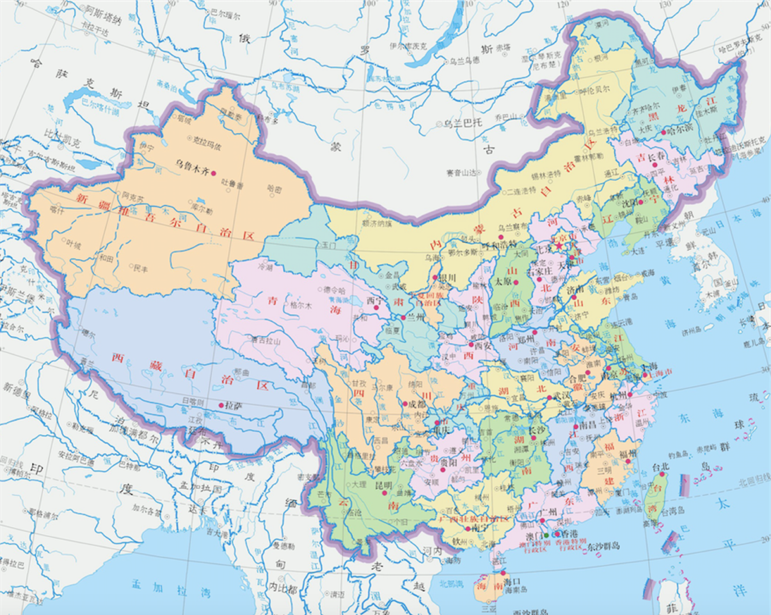
\includegraphics[width=0.8\textwidth]{ConfucianismeTaoismeBouddhismeChinois/Images/CarteChine.png}

    \label{fig:enter-label}
\end{figure}
\paragraph{34 provinces} dont Taiwan. 3 paliers, le Tibet, à l'Est, les plaines et au milieu, en diagonale, des moyenne montagne. L'économie suit
\begin{marginfigure} 
    \centering
        \caption{Relief Chinois}
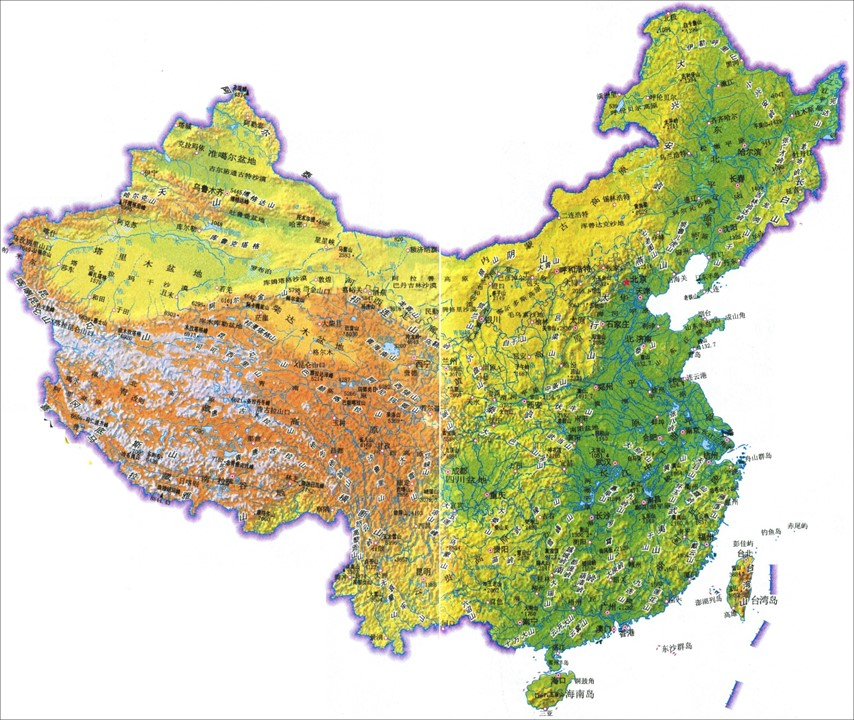
\includegraphics[width=\textwidth]{ConfucianismeTaoismeBouddhismeChinois/Images/CarteChineRelief.jpg}

    \label{fig:enter-label}
\end{marginfigure}

 

\paragraph{Les fleuves} Le fleuve Jaune (Huanghe), car Loess. au sud, le Changjiang, le fleuve long, appelé en français, le fleuve bleu.


\section{Histoire}
\paragraph{chronologie} une vieille histoire mais mouvementée. Relu en fait par les nouveaux envahisseurs pour s'approprier le payes. 

\paragraph{- 221 av JC : l'Empire de Qin} centralisé, avec une bureaucratie.

\paragraph{1911} dernier empire est renversé
\paragraph{1949} république populaire de la Chine.

\subsection{Chronologie}
\begin{figure}[!h]
    \centering
        \sidecaption{Chronologie -Corinne Debaine-Francfort, La redécouverte de la Chine ancienne, Paris: Gallimard, 1998, p. 142-148}
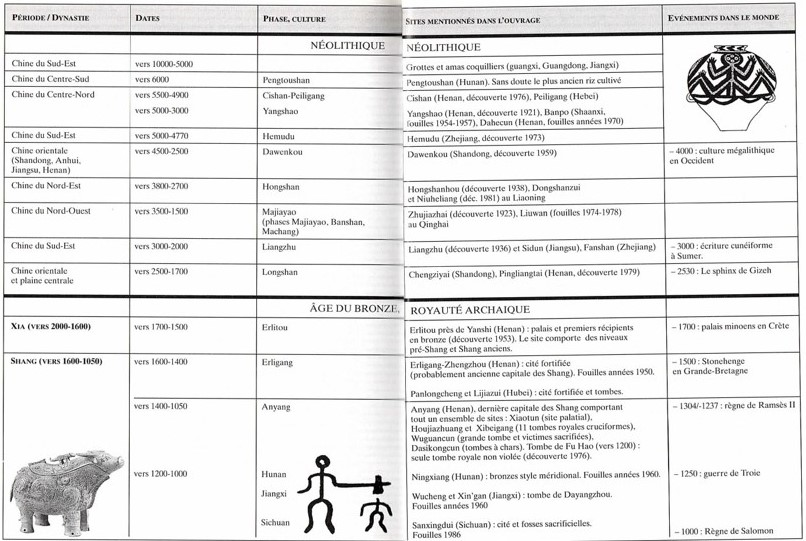
\includegraphics[width=0.8\textwidth]{ConfucianismeTaoismeBouddhismeChinois/Images/Chronologie1.jpg}
\includegraphics[width=0.8\textwidth]{ConfucianismeTaoismeBouddhismeChinois/Images/Chronologie2.png}
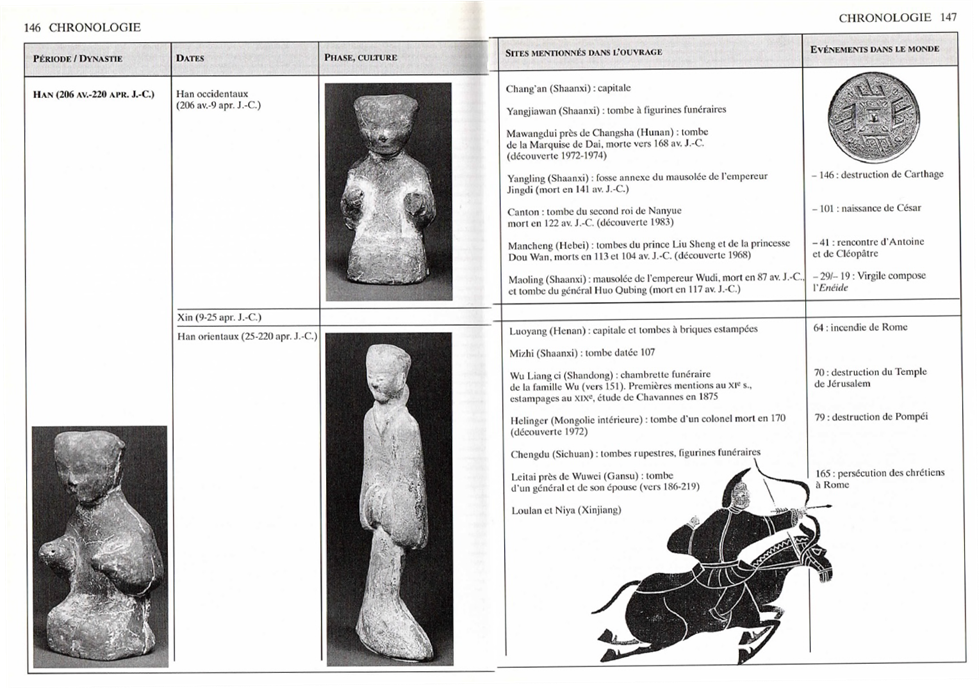
\includegraphics[width=0.8\textwidth]{ConfucianismeTaoismeBouddhismeChinois/Images/Chronologie3.png}

    \label{fig:enter-label}
\end{figure}

\FloatBarrier

\paragraph{les dynasties} Superficiellement, on peut avoir l'impression d'une stabilité avec un cycle "mauvaise récolte, révolte, changement de dynastie". Mais c'est ignorer ce que chaque dynastie apporte à commencer par la façon de recruter les fonctionnaires.


\begin{Prop}[les dynasties et l'écriture]
    Les dynasties chinoises marquent parfois de grandes discontinuité. Elles sont étroitement liées à la méthode de gouverner et à l'écriture.
\end{Prop}

\paragraph{rapport entre l'homme et l'espace} Comment l'homme arrive à s'installer sur le territoire. 

\paragraph{l'homme de pékin, \textit{homo erectus}} Hommes de Pékin: premiers hommes de Chine (700,000– 30,000 AEC)

\paragraph{révolution néolithique 5000-3000 av JC} on peut s'installer grâce au stockage liée à la poterie.
Grâce à Andersson au XIX, les poteries à Stockholm.
\begin{figure}[!h]
    \centering
        \sidecaption{Neolithique Ancien}
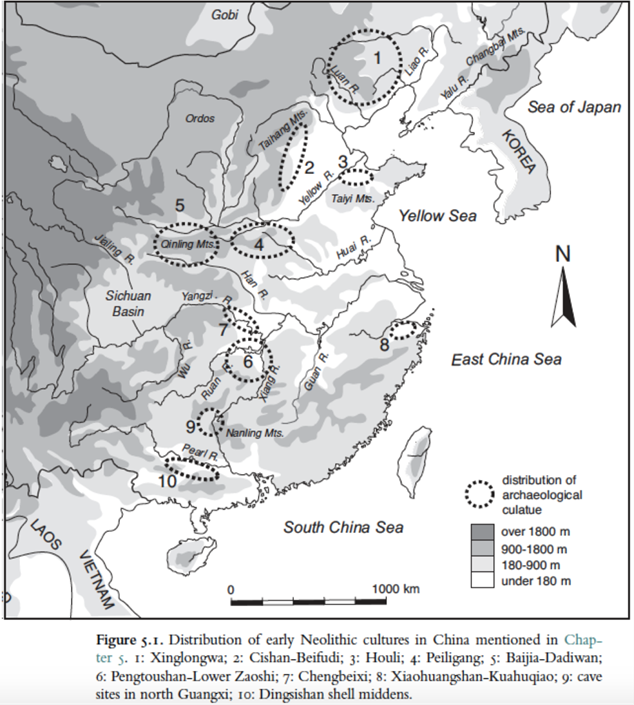
\includegraphics[width=0.6\textwidth]{ConfucianismeTaoismeBouddhismeChinois/Images/NeolithiqueAncien.png}

    \label{fig:enter-label}
\end{figure}

\paragraph{Néolithique moyen}


 
\begin{marginfigure}
    \caption{Exemple de Vase Néolithique Tardif - Musée National de Chine}
    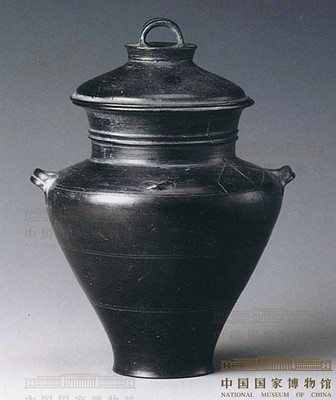
\includegraphics[width=\textwidth]{ConfucianismeTaoismeBouddhismeChinois/Images/NeolithiqueTardifNationalMuseum.jpg}

\end{marginfigure}
\FloatBarrier
\paragraph{néolithique tardif 3000-2000 av JC} des objets en jade. Hierarchisation de la société. première forme d'Etat.
\begin{figure}[!h]
    \centering
        \caption{Neolithique Tardif
        Source: Liu Li (2012), p. 124.}
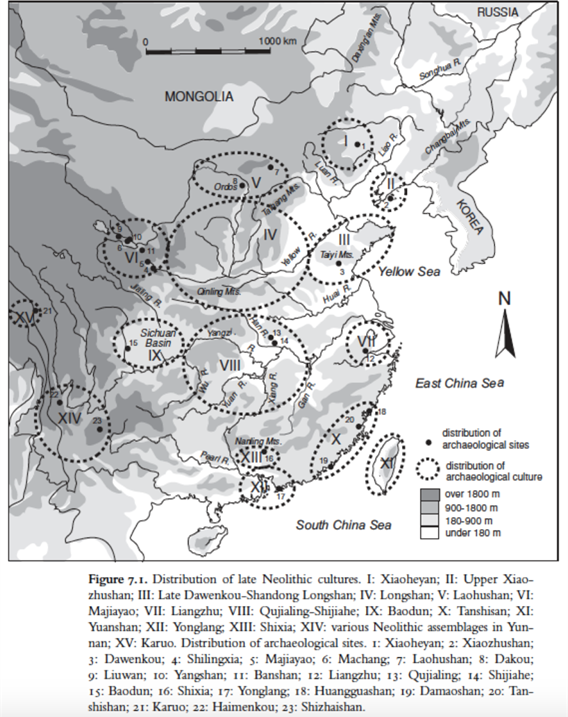
\includegraphics[width= .6\textwidth]{ConfucianismeTaoismeBouddhismeChinois/Images/NeolithiqueTardif.png}

    \label{fig:enter-label}
\end{figure}



\FloatBarrier
\subsection{Origine de la Chine : singulière ou plurielle ?}
\paragraph{une question : Chine singulière ou plurielle} \textit{Zhong gao} : Empire du Milieu, appelation très ancienne. Pourrait faire penser à un noyau, un centre qui aurait irradié autour. Mais les découvertes archéologiques mettent en question cette interprétation. 

\begin{marginfigure}
        \centering
        \caption{Modèle« Chinese interaction sphere » Proposé par K. C. Chang en 1986}
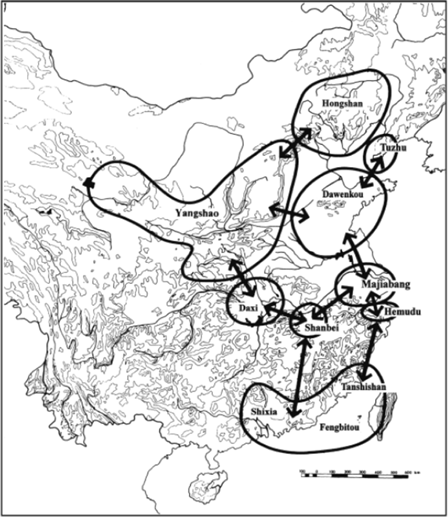
\includegraphics[width=\textwidth]{ConfucianismeTaoismeBouddhismeChinois/Images/ModeleChineseInteractionSphere.png}
\end{marginfigure} 


\FloatBarrier
\subsection{Dynastie Shang et le début de l'écriture chinoise}

\paragraph{dynastie Shang (1250-1055 av JC} culture dominante dans l'aire autour de Anyang. premières traces de l'écriture, les \textit{jiaguwen}

\begin{figure}[!h]
    \centering
        \sidecaption{Les différentes cultures ayant existé durant la phase tardive des Shang (1250-1050 AEC) Source: Li Feng (2013), p. 84}
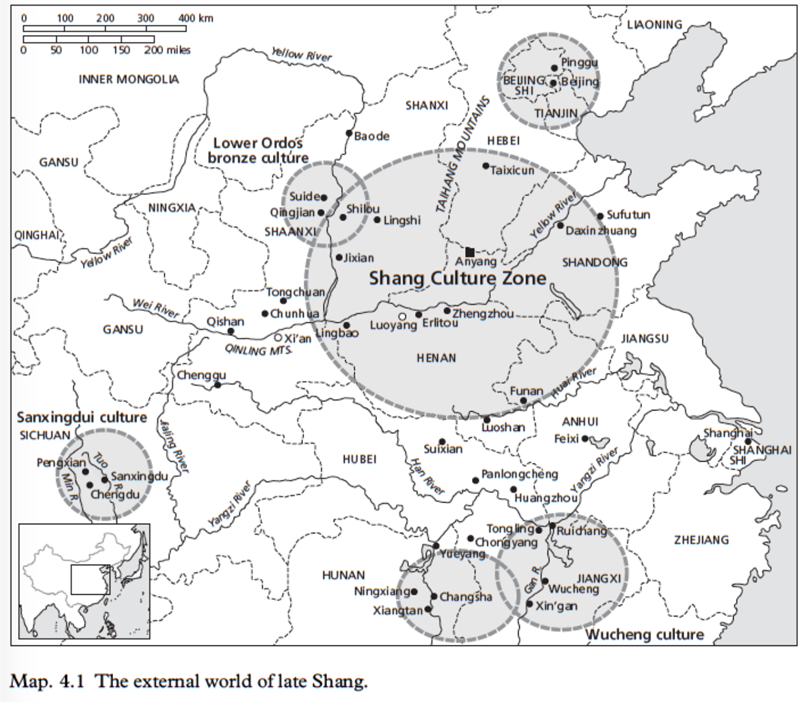
\includegraphics[width=0.8\textwidth]{ConfucianismeTaoismeBouddhismeChinois/Images/EmpireShang.png}

    \label{fig:enter-label}
\end{figure}

 \FloatBarrier
\paragraph{les Jiaguwen}
\begin{Def}[Jiaguwen]
    inscriptions oraculaires sur carapaces de tortue et os.
    \textbf{Divinatoire}
\end{Def}


\begin{figure}[!h]
    \centering
        \sidecaption{Exemple de Jiaguwen inscriptions oraculaires sur carapaces de tortue et os}
\includegraphics[width=0.8\textwidth]{ConfucianismeTaoismeBouddhismeChinois/Images/CarapaceEcriture.png}

    \label{fig:enter-label}
\end{figure}
\begin{Ex}
    On pose des questions à Dieu : "est ce que j'aurais une bonne récolte ?"
On fait chauffer la carapace et on interprète la craquelure (orientation et sur quel mot). 
\end{Ex}

\paragraph{Même structure} préface (quel jour on a posé la question) + quelle question (charge) + oracle proprement dit. 
\begin{figure}[!h]
    \centering
        \sidecaption{Exemple de lecture}
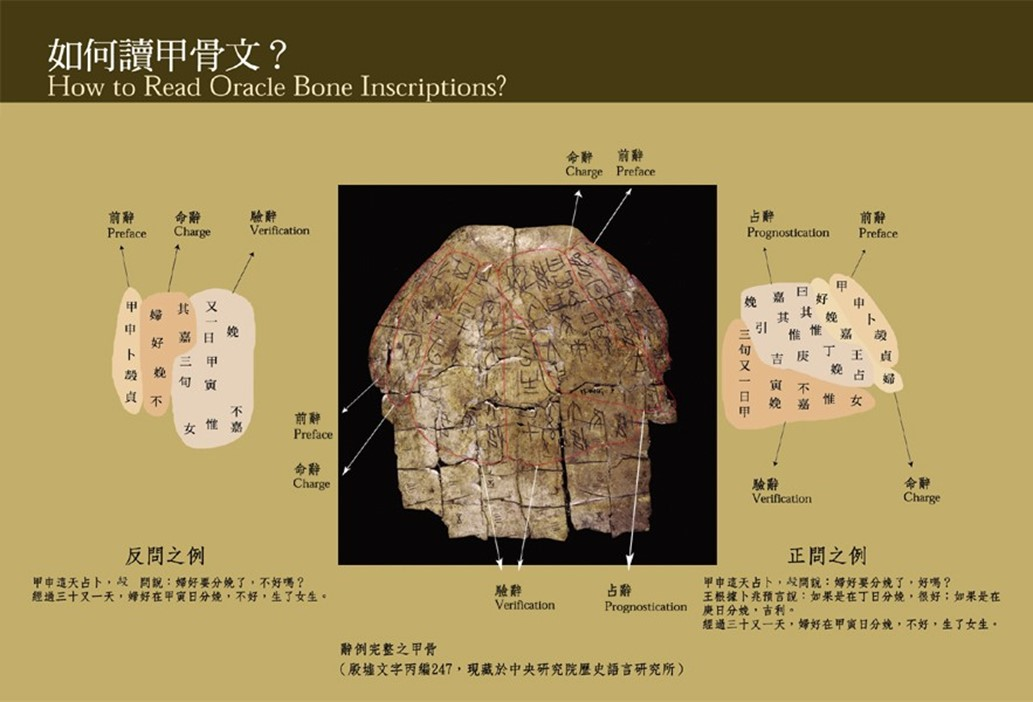
\includegraphics[width=0.8\textwidth]{ConfucianismeTaoismeBouddhismeChinois/Images/ReadOracle.jpg}

    \label{fig:enter-label}
\end{figure}

\subsection{la dynastie des Zhou}
on dit : "djzo"
\begin{figure}[!h]
    \centering
        \sidecaption{Carte des Zhous Occidentaux}
\includegraphics[width=0.8\textwidth]{ConfucianismeTaoismeBouddhismeChinois/Images/ZhouOccidentaux.png}

    \label{fig:enter-label}
\end{figure}

\paragraph{Equivalent du féodalisme en occident} Le roi octroie des territoires à ces membres de familles.  des Bronzes marquant la différence entre roi, prince,...


\paragraph{lien de suzeraineté} le roi donne un bronze qui marque la suzeraineté et les remerciements du roi. On les met dans le temple des ancêtres. Souvenir pour les générations suivantes
\begin{marginfigure}
    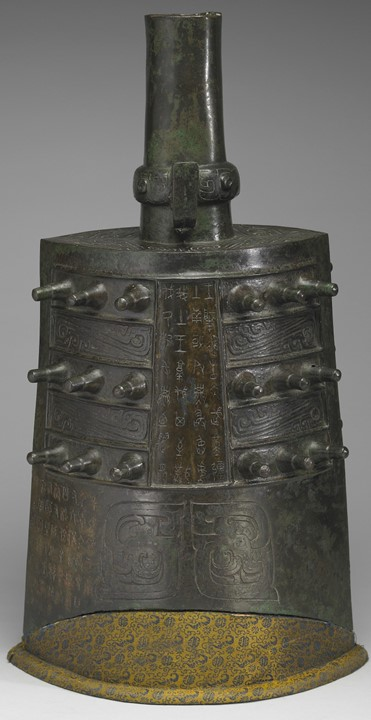
\includegraphics[width=\textwidth]{ConfucianismeTaoismeBouddhismeChinois/Images/ZhouBronze.jpg}
\end{marginfigure}
\paragraph{le mandat céleste} Le roi croit dans le fait qu'ils ont un mandat de Dieu et qu'ils peuvent condamner.

\paragraph{Obligation de diviser le territoire} pour octroyer des terres car plus de marche. Affaiblissement économique des Rois Zhou.
Les territoires des marches arrivent à s'aggrandire (les chu, les qin,...) et deviennent de plus en plus puissants. 

\paragraph{la grande muraille} 


\paragraph{Les Etats indépendants} avant l’unification de l’empire en 221 avant notre ère
\begin{figure}[!h]
    \centering
        \sidecaption{Carte des Etats indépendants  256 av JC}
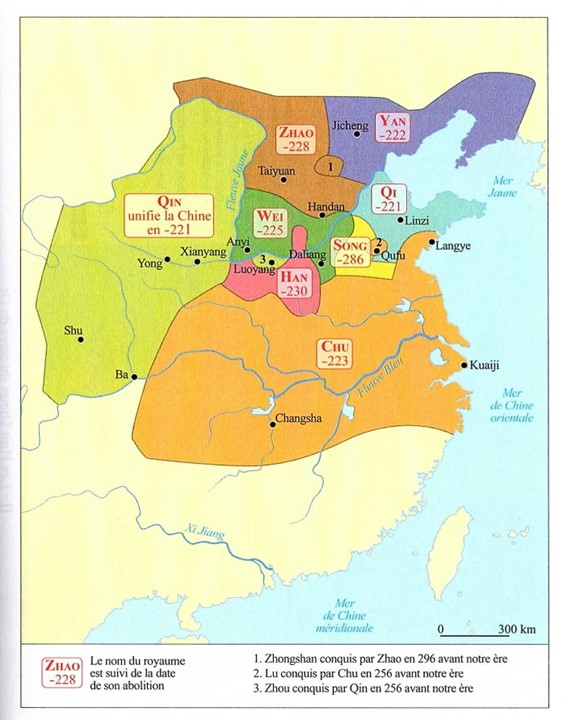
\includegraphics[width=0.5\textwidth]{ConfucianismeTaoismeBouddhismeChinois/Images/CarteEtatsIndependants.jpg}

    \label{fig:enter-label}
\end{figure}


\subsection{L'empire des Qin et des Han }
\paragraph{Qin} ne dure pas longtemps '221-206

\begin{marginfigure}
    \centering
        \caption{L'empire des Qin}
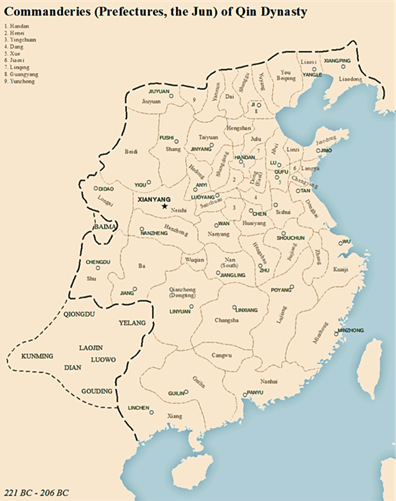
\includegraphics[width= \textwidth]{ConfucianismeTaoismeBouddhismeChinois/Images/CarteQin.png}

    \label{fig:enter-label}
\end{marginfigure}

\paragraph{Les Hans : arrêtent l'allocation de terres mais installent bureaucratie} Centralisation. et Standardisation des poids et mesures.Une monnaie unique. 
\begin{marginfigure} 
    \centering
        \caption{La dynastie des Han  /  (202 av. J.-C. - 220 apr. J.-C.)}
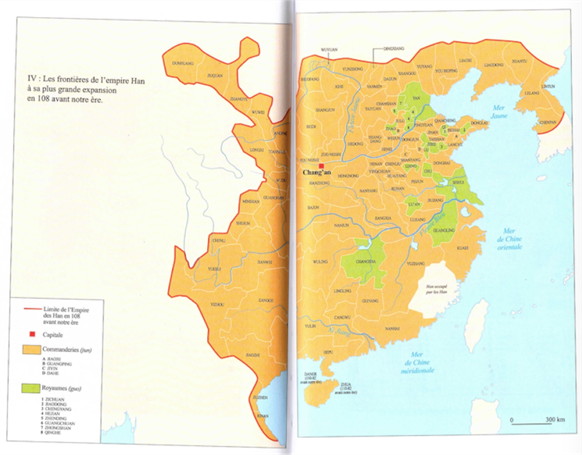
\includegraphics[width=\textwidth]{ConfucianismeTaoismeBouddhismeChinois/Images/CarteHan.png}

    \label{fig:enter-label}
\end{marginfigure}
\paragraph{Standardisation de l'Ecriture} Ce sont majoritairement les scribes qui écrivent. Sur les tablettes et manuscrit, on passe à la variante vulgaire des \textit{Qin. } {comme en grec, le Sigma qui devient C}


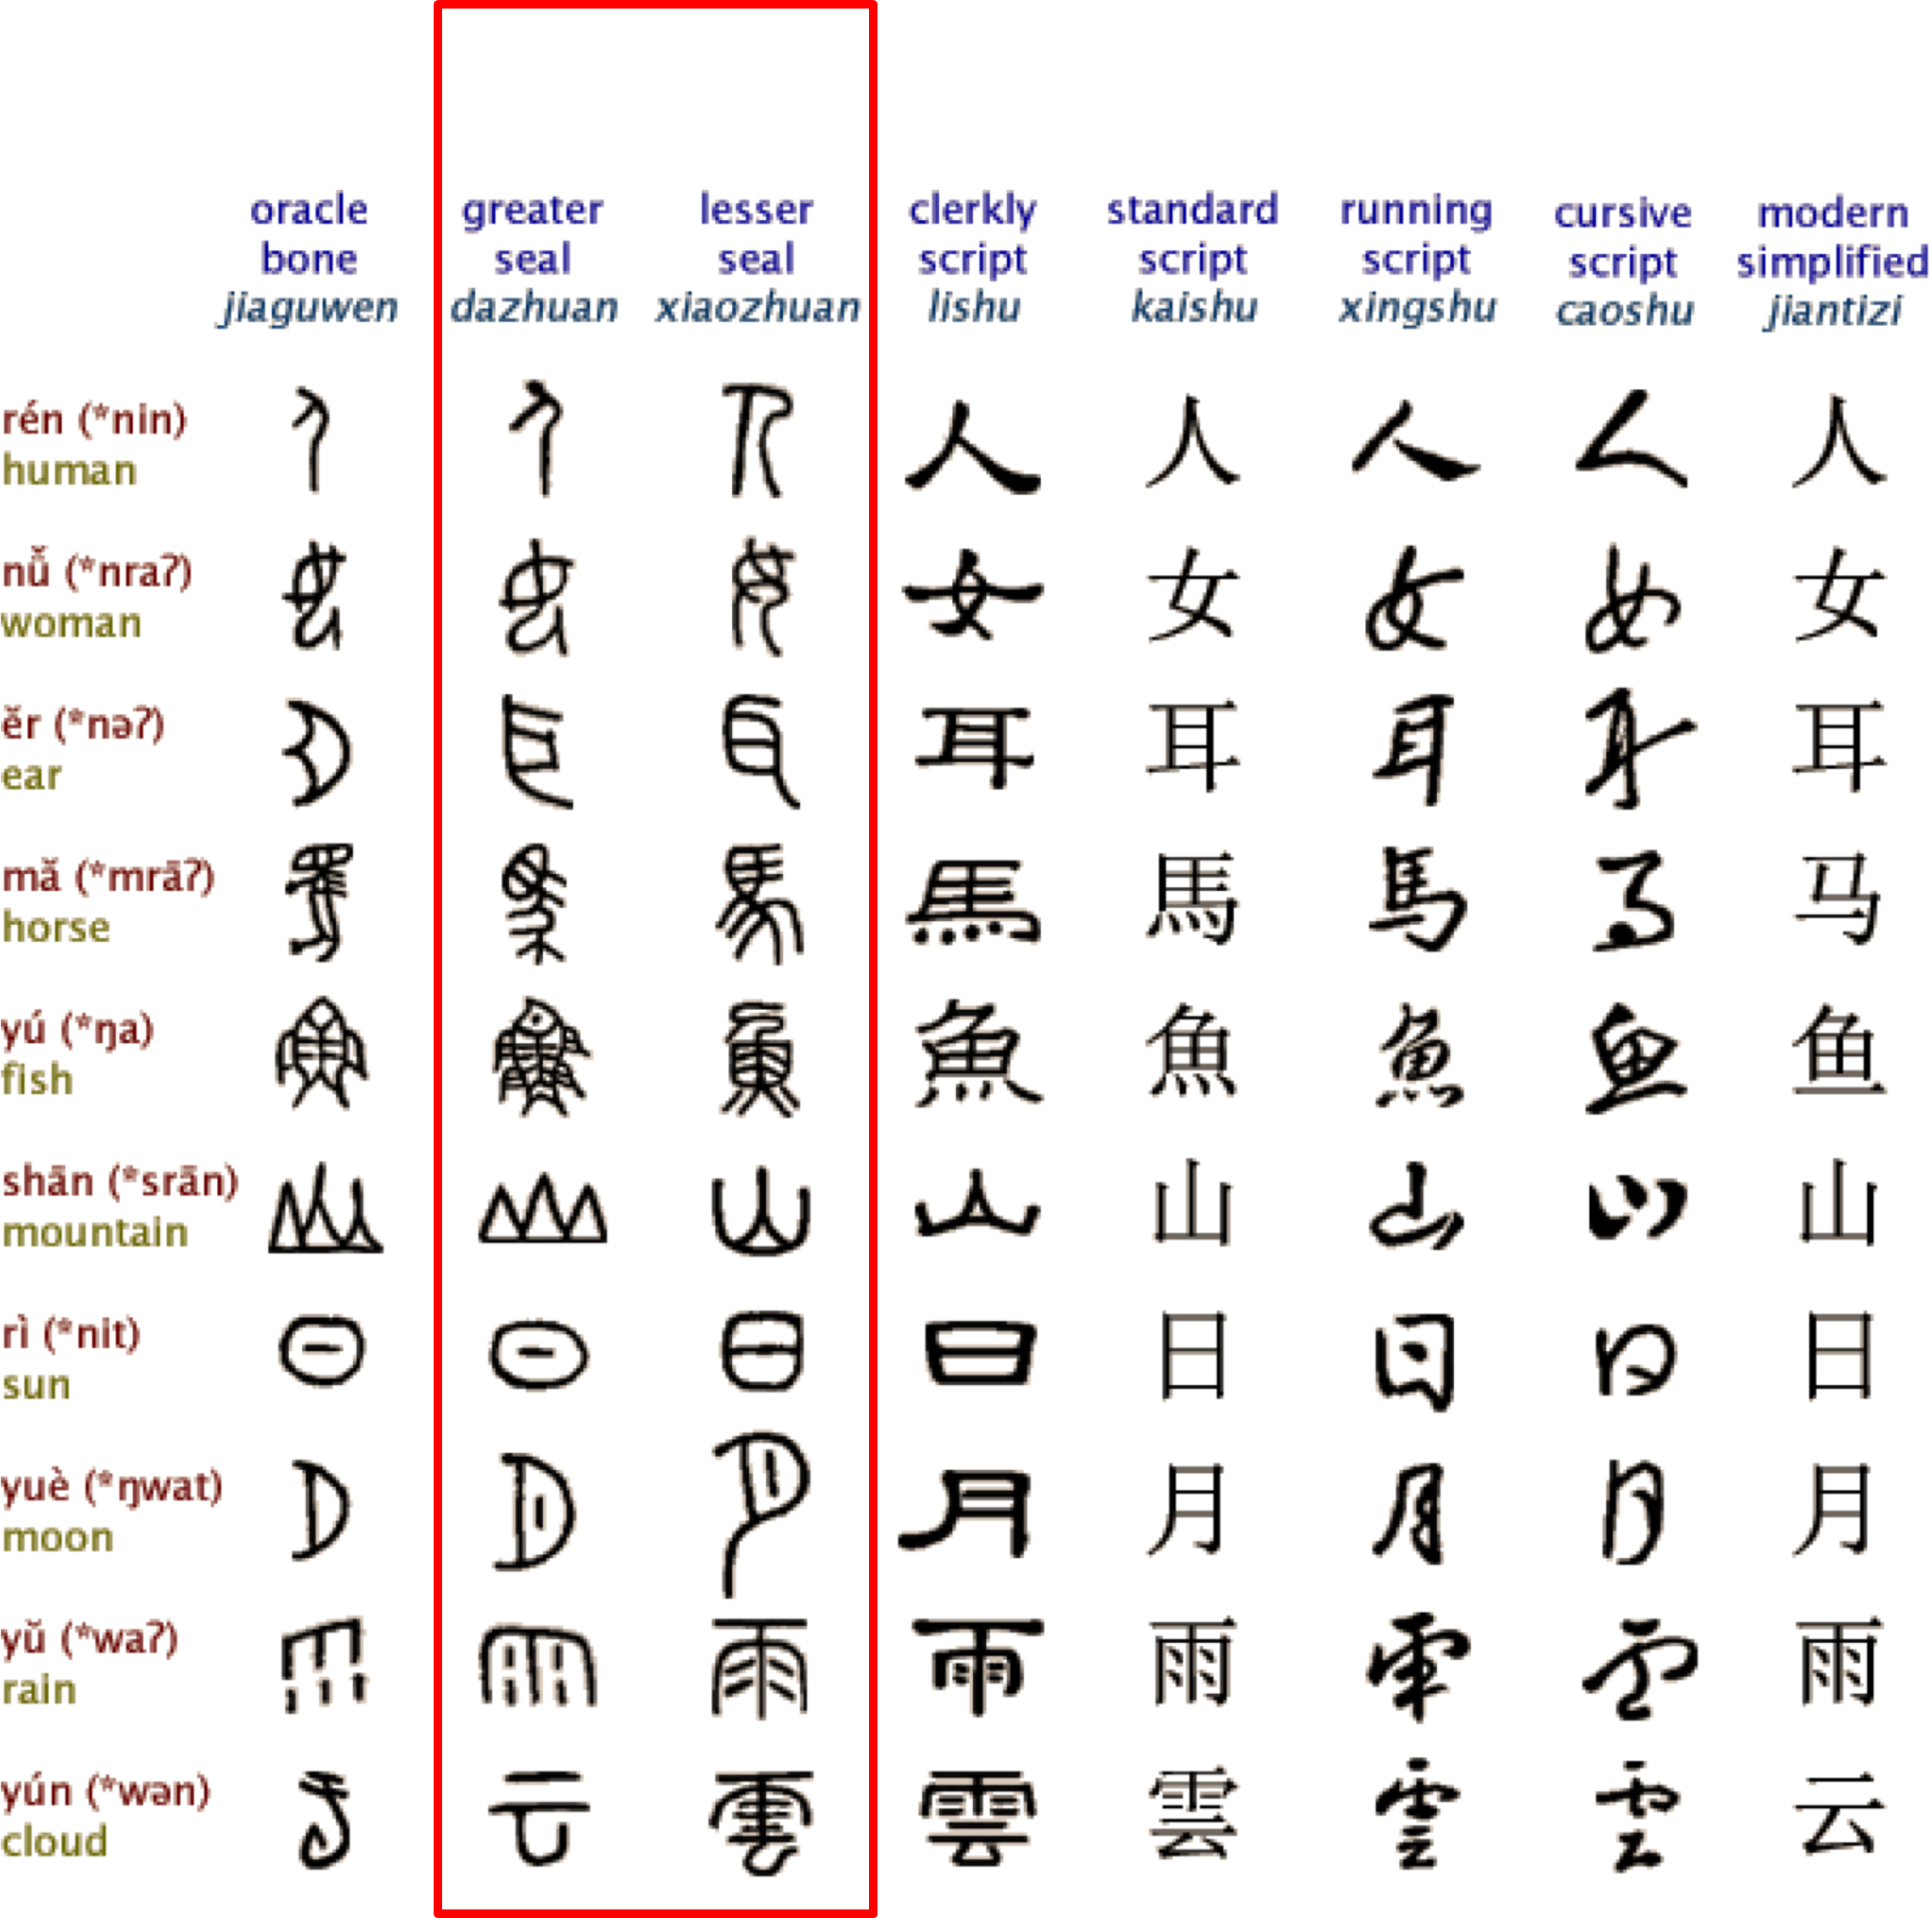
\includegraphics[width=0.8\textwidth]{ConfucianismeTaoismeBouddhismeChinois/Images/StandardisationEcritureQin.png}


\paragraph{Exemple de simplification de l'écriture} On voit l'arrondi des lettres de la petite sigilaire à leur variante vulgaire\sn{Zhitang Yang-Drocourt, L’écriture chinoise, Malakoff: Armand Colin, 2022, p. 57.}. 


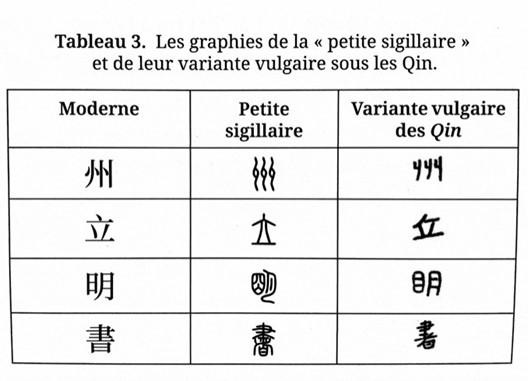
\includegraphics[width=0.8\textwidth]{ConfucianismeTaoismeBouddhismeChinois/Images/QinEcritureExemple.jpg}

\paragraph{période de mélange ethnique très important} d'où le fait que le nom de la dynastie donne le nom à la population \textit{Han}. 

\paragraph{Les Hans} analysent pourquoi les Qin n'ont pas duré. Constat que c'est parce qu'ils gouvernent par les lois et non les vertus.

\paragraph{Arrivée du Bouddhisme} à la fin de la dynastie Han. 
Une véritable création pour trouver dans la langue chinoise des termes pour traduire les termes bouddhiques. 

\paragraph{Vème siècle} On écrit sur du papier et non de la soie, du bambou. On écrit avec le pinceau. 


\paragraph{Comment la dynastie Han a donné son nom au peuple Han} Le déplacement des peuples non-Han sous les six dynasties (220 – 589)
\begin{marginfigure}
    \includegraphics[width=\textwidth]{ConfucianismeTaoismeBouddhismeChinois/Images/DeplacementNonHan.png}
\end{marginfigure}
Pendant cette période, le terme « Han»  qui était au départ le nom d’une dynastie commençait à être utilisé pour désigner la population indigène, c’est-à-dire les chinois, afin de les distinguer des populations étrangères.

Aujourd’hui, le terme Han désigne encore le groupe ethnique majoritaire de la Chine. (hanzu  )
\paragraph{Période de chaos?
}

% ---------------------------------------------------
\subsection{La dynastie des Tang 618-907}
\begin{figure}
    \centering
        \sidecaption{La dynastie des Tang  (618-907)}
    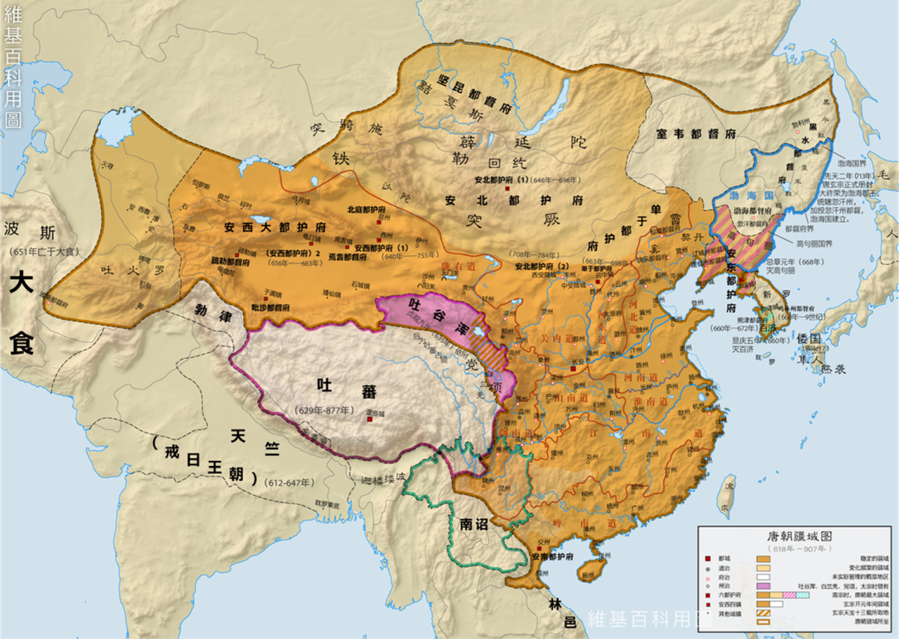
\includegraphics[width=\textwidth]{ConfucianismeTaoismeBouddhismeChinois/Images/CarteTang.png}

    \label{fig:enter-label}
\end{figure}
\paragraph{bcp d'échange avec l'Asie centrale - route de la soie}

\paragraph{Ecole Shan bouddhique} en Japonais, Zen. On se concentre sur la méditation.


\subsection{La dynastie des Song}
\begin{figure}
    \centering
        \sidecaption{La dynastie des Song}
    \includegraphics[width=\textwidth]{ConfucianismeTaoismeBouddhismeChinois/Images/CarteSong.png}

    \label{fig:enter-label}
\end{figure}
\paragraph{La dynastie des Song du Nord}
 
\paragraph{Néo confucianisme}

\subsection{La dynastie Yuan} 

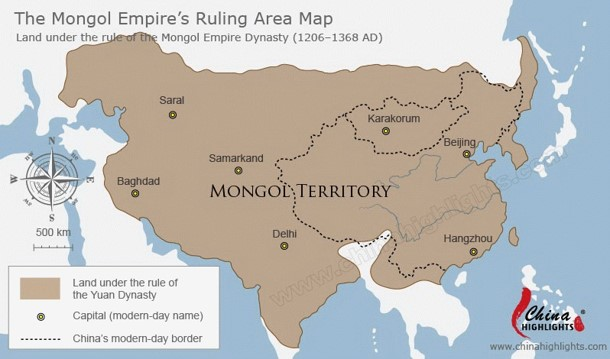
\includegraphics[width=0.6\textwidth]{ConfucianismeTaoismeBouddhismeChinois/Images/CarteYuan.jpg}
\paragraph{La dynastie des Yuan}  (1271 - 1368) faisait partie de l’Empire mongol fondé par Gengis Khan (r. 1206- 1227). Son petit fils, Kubilaï, fonda en 1271 la dynastie des Yuan.

\paragraph{fait partie de l'empire Mongol}

\subsection{Dynastie des Ming}
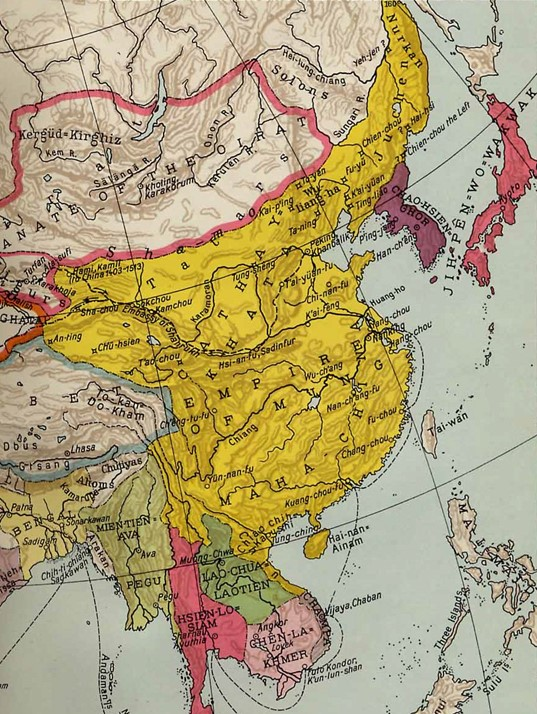
\includegraphics[width=0.6\textwidth]{ConfucianismeTaoismeBouddhismeChinois/Images/CarteMing.jpg}
\paragraph{dynastie des Ming} (1368-1644)


\subsection{Dynastie des Qing et chronologie récente}

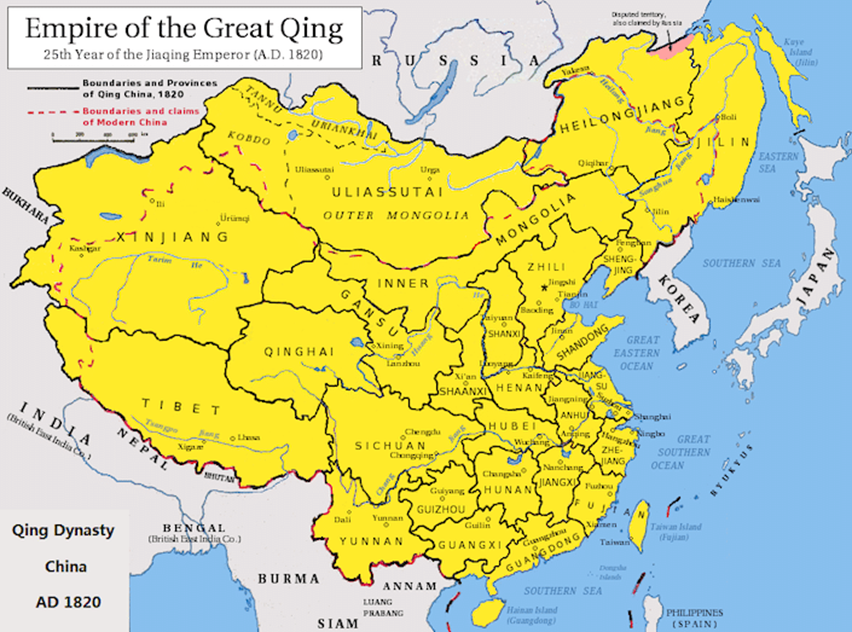
\includegraphics[width=0.6\textwidth]{ConfucianismeTaoismeBouddhismeChinois/Images/CarteQing.png}
\paragraph{la dynastie des Qing}  (1644-1911) dynastie Mandchoue de nouveau allogène. 


\begin{figure}[!h]
    \centering
        \sidecaption{Chronologie récente}
\includegraphics[width=0.9\textwidth]{ConfucianismeTaoismeBouddhismeChinois/Images/Chronologie4.png}
    \label{fig:enter-label}
\end{figure}

\subsection{le cours}

\paragraph{les trois enseignements (jiao)} qu'on utilisait avant à la place du mot \textit{religion}
Qu'est ce qu'un enseignement, avant de parler de religion ?




